\documentclass[a4paper,11pt]{report}
\usepackage[T1]{fontenc}
\usepackage[utf8]{inputenc}
\usepackage{lmodern}
\usepackage{color}
\usepackage{graphicx}
\graphicspath{ {images/} }
\usepackage{hyperref}

\title{Udacity Stroop Effect Experiment}
\author{Neil Seas}

\begin{document}

\maketitle
\tableofcontents

\begin{abstract}
This document answers the \href{https://docs.google.com/document/d/1-OkpZLjG_kX9J6LIQ5IltsqMzVWjh36QpnP2RYpVdPU/pub?embedded=True}{questions} posed in Project 1 of the Udacity Data Analyst Nanodegree program.  Its purpose is to practice with basic concepts of statistical testing.  In particular, testing for statistical significance of a sample set of data for people taking the Stroop test.
\end{abstract}

\chapter{Questions}
\section{Question 1}
  \begin{itemize}
    \item \textbf{What is the \textit{independent variable}?}\\
    The test measures the time it takes to say a list of colored words, where the goal is to say the color of the word and not the color spelled by the word.  This task is performed twice by the same subject, which means we are working with dependent samples.  In the \textbf{congruent} case the words and the colors of the words match (e.g. \textcolor{green}{GREEN}).  In the \textbf{incongruent} case the words and the colors of the words do not match (e.g. \textcolor{red}{GREEN}).

The \textbf{independent variable} can take on two values: congruent or incongruent.  The \textbf{dependent variable} is the time it takes to read the color of each word in the list measured in seconds.
  \end{itemize}

\section{Question 2}
  \begin{itemize}  
    \item \textbf{What is an appropriate set of hypothesis for this task?  What kind of statistical test do you expect to perform?}\\
    Intuitively, it seems that the \textbf{incongruent} list would take longer than the \textbf{congruent} list to read.  Trying to separate the color from the written word would seem to demand more attention and therfore more time.  Given that our expectation for the difference in means has a direction a \textbf{one-tailed} test was chosen.  Since this is a sample and the population parameters are unknown we will use a \textbf{t-test} to evaluate statistical significance.  

    Null Hypothesis: \( H_0: \mu_C = \mu_I \)\\
    Alternative Hypothesis: \( H_1: \mu_C < \mu_I \)\\
    
    Because the sample is a dependent sample I am using the following formulation for the standard deviation: \\
    \begin{center}
      \( \sqrt{S_C^2 + S_I^2} \)\\
    \end{center}
    where \( S_C^2 \) is the variance of the congruent test results and \( S_I^2 \) is the variance of the incongruent test results.\\
  \end{itemize}
  
\section{Question 3}
  \begin{itemize}
    \item \textbf{Report some descriptive statistics regarding this dataset.  Include at least one measure of central tendency and at least one measure of variability}\\
    \begin{center}
      \begin{tabular}{|| l c c ||}
      \hline
      & Congruent & Incongruent \\
      \hline\hline
      Sample Size & 24 & 24 \\
      \hline
      Sample Mean & 14.05 & 22.02 \\
      \hline
      Median & 14.36 & 21.02 \\
      \hline
      Sample StDev & 3.56 & 4.80 \\
      \hline
      \end{tabular}
    \end{center}
  \end{itemize}
  
\section{Question 4}
  \begin{itemize}
    \item \textbf{Provide one or two visualizations that show the distribution of the sample data.  Write one or two sentences noting what you observe about the plot(s)}\\
    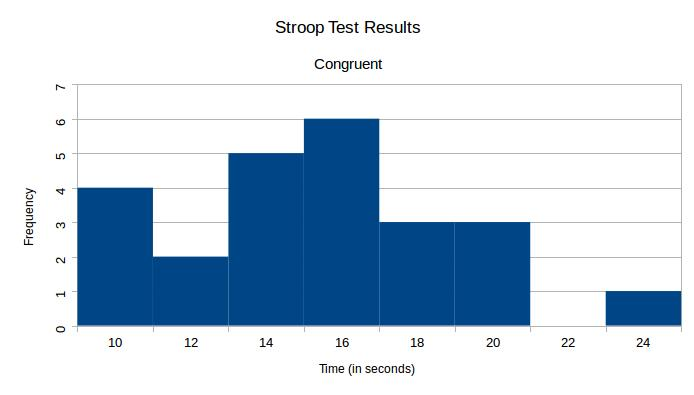
\includegraphics[scale=.5]{congruent_histogram}\\
    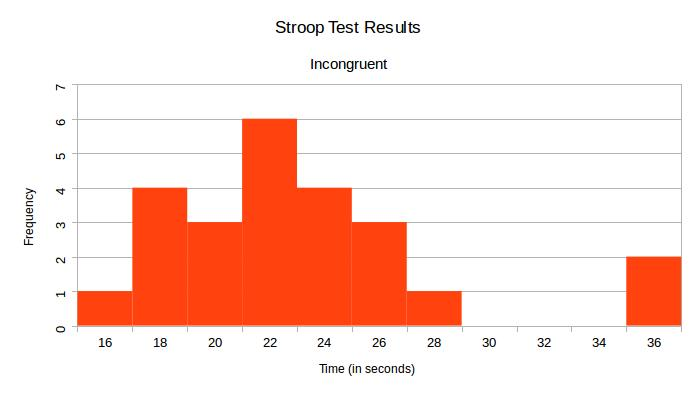
\includegraphics[scale=.5]{incongruent_histogram}\\
    The sample size is rather small, but there is still a relatively normal shape to both distributions.  In both the congruent and incongruent samples there are outliers above the mean.
  \end{itemize}
  
\section{Question 5}
  \begin{itemize}
    \item \textbf{Now, perform the statistical test and report your results. What is your confidence level and critical statistic value?}
    \begin{center}
      \begin{tabular}{|| l c||}
      \hline
      & Results \\
      \hline\hline
      alpha level & .05 \\
      \hline
      critical t & -1.714 \\
      \hline
      t statistic & -6.532 \\
      \hline
      \end{tabular}
    \end{center}
    
    \item \textbf{Do you reject the NULL hypothesis or fail to reject it?}
    Given the critical value of t and the calculated t statistic we will reject the NULL hypothesis and accept the alternative hypothesis that \( \mu_C < \mu_I \).
    \item \textbf{Come to a conclusion in terms of the experiment task.  Did the results match up with your expectations?}
    The results provide strong evidence that the mean time to complete the incongruent version of the test take longer than the congruent test.  The t statistic calculated from our sample suggest that our result is extremely statistically significant.  The P value for the calculated t statistic and 23 degrees of freedom is less than .0001.
    
  \end{itemize}
  
\section{Question 6 Optional}
  \begin{itemize}
    \item \textbf{What do you think is responsible for the effects observed?  Can you think of an alternative or similar task that would result in a similar effect?}\\
    Based on a brief reading of the Wikipedia page for the \href{https://en.wikipedia.org/wiki/Stroop_effect}{Stroop Effect} it seems that there are a few theories about why the Stroop effect occurs.  Broadly speaking, the effect seems to come about because it requires the brain to do parallel processing.  The resulting time difference between tasks could be due to the difficulty of filtering out distracting information or due to our brains having stronger pathways for processing words than colors.  It strikes me that any number of tasks could be tested for the Stroop effect.  Any task could be performed without distraction and then performed again with some sort of distraction.
  
  \end{itemize}
  
\section{Sources Used}
  \begin{itemize}
    \item Udacity lectures
    \item Wikipedia
    \item GraphPad (for calculating P value of result)
  \end{itemize}
\end{document}
